
\section{Solutions for ``Isomorphisms of Groups''}
\noindent\textbf{\textit{ (Chapter \ref{isomorph}})}\bigskip
\\
\textbf{Exercise \ref{exercise:isomorph:iso_1}:} 
$f(r \cis \theta) = (r\cos \theta, r \sin \theta )$
\\
\textbf{Exercise \ref{exercise:isomorph:iso_2}:}
%Prove that the function $f$ defined in Example~\ref{example:isomorph:chap1_ex}  is a bijection.
%\\
Proof: To show it's a  bijection we may prove that it's 1:1 and onto.  However, it's much simpler just to show that 
$f$ has an inverse:  $f^{-1}( (a,b) ) = a + bi$.  We've shown previously that a function is a bijection iff it has an inverse.
\\
For your cultural enrichment, a direct proof that $f$ is a bijection runs as follows.
Let $f : {\mathbb C} \longrightarrow {\mathbb R} \times {\mathbb R}$ be defined as $f(a + bi) = (a,b)$ for all $a +  bi \in {\mathbb C}$ where $a, b \in {\mathbb R}$
\\
For 1:1, let $a + bi, c + di \in {\mathbb C}$
\begin{align*}
f(a + bi) &= f(c + di) &\text{(by supposition)}
\\
(a, b) &= (c, d) &\text{(def of\ } f)
\\
\implies a &= c \text{\ and\ } b = d &(\text{Definition~\ref{orderedpair}})
\end{align*}
Therefore, $f$ is 1:1.
\\
\\
Now, given that $(a, b) \in {\mathbb R} \times {\mathbb R}$, there exists some $a + bi \in {\mathbb C}$ such that $f(a + bi) = (a, b)$
\\
Therefore $f$ is onto.
\\
Since $f$ is 1:1 and onto, $f$ is a bijection.
\\\\

\noindent\textbf{Exercise \ref{exercise:isomorph:iso_3}:}
%Draw a diagram similar to Figure~\ref{fig:groups:CommDiag}  for the function $g: {\mathbb C} \rightarrow {\mathbb R} \times {\mathbb R}$ defined by $g(a + bi) = (3a, 3b)$. Show that the same ``arrow-following'' property holds: that is, you can follow the arrows from the upper left to lower right in either order, and still end up with the same result.
\\
\begin{figure}[H]
	   \center{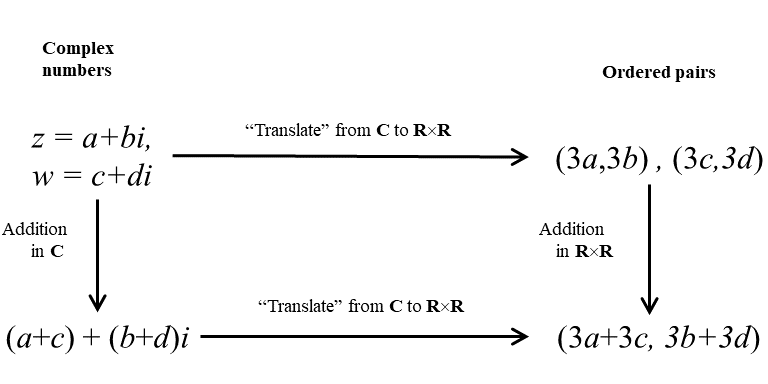
\includegraphics[width=4.in]
	         {images/CommDiagIso3.png}}
\end{figure}

\noindent\textbf{Exercise \ref{exercise:isomorph:iso_4}:}
%Prove that the function $h(a + bi) = (a+2, b+2)$ is {\bf not} an isomorphism from ${\mathbb C}$ to  ${\mathbb R} \times {\mathbb R}$.
%\hyperref[sec:isomorph:hints]{(*Hint*)}
%\\
\begin{figure}[H]
	   \center{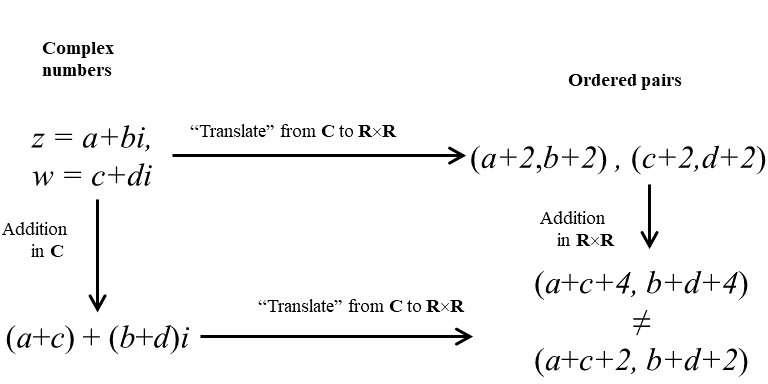
\includegraphics[width=4.in]
	         {images/CommDiagIso4.png}}
\end{figure}
Counterexample: Let $z = 3 + 4i, w = 2 + i \in {\mathbb C}$
\begin{align*}
\text{Then\ } z + w &= (3 + 4i) + (2 + i) &\text{(by substitution)}
\\
&= (3 + 2) + (4 + 1)i &\text{(complex addition)}
\\
&= 5 + 5i &\text{(basic algebra)}
\\
h(z + w) &= h(5 + 5i) &\text{(function of h)}
\\
&= (5 + 2, 5 + 2) &\text{(def of h)}
\\
&= (7, 7) &\text{(algebra)}
\\
h(z) + h(w) &= h(3 + 4i) + h(2 + i) &\text{(by substitution)}
\\
&= (3 + 2, 4 + 2) + (2 + 2, 1 + 2) &\text{(by def of h)}
\\
&= (5, 6) + (4, 3) &\text{(by algebra)}
\\
&= (5 + 4, 6 + 3) &\text{(by addition)}
\\
&= (9, 9) &\text{(algebra)}
\end{align*}
but $h(z + w) = (7, 7) \neq (9, 9) = h(z) + h(w)$
\\
so $h$ is not an isomorphism
\\
\\

\noindent\textbf{Exercise \ref{exercise:isomorph:iso_7}:}
%Determine whether each of the following functions are isomorphisms between the groups in Example~\ref{example:isomorph:sym_ex}. Justify your answers. 
\begin{enumerate}[(a)]
\item
%$ f: {\mathbb Z_4}  \longrightarrow \langle i \rangle$ defined by 
%\[  
%f(0) = 1,~~
% f(1) = -1,~~
% f(2) = i,~~
% f(3) = -i.
%\]
To show that $f$ is not an isomorphism, it is sufficient to find one example where the isomorphism relation fails.
We have:  $f(1+1) = f(2) = i$  but $f(1) \cdot f(1) = (-1)(-1) = 1$.  It follows that $f(1+1) \neq f(1)\cdot f(1)$, so $f$ is not an isomorphism.

\item
%$ g: {\mathbb Z_4}  \longrightarrow R_4$ defined by 
%\[ 
%g(0) = \var{id},~~
%g(1) = r_{270},~~
%g(2) = r_{90} ,~~
%g(3) = r_{180}. 
%\]
Verify that $g(1+1) \neq g(1)\cdot g(1)$, which shows that $g$ is not an isomorphsim.\\

\item
The Cayley table for $\langle i \rangle$ is:

\begin{multicols}{2}
\begin{table}[H]
{\small
\begin{center}
\begin{tabular}{c|cccccccc}
$\cdot$ & 1 & i & -1 & -i  \\
\hline
1        & 1 & i & -1 & -i  \\
i       & i & -1 & -i & 1  \\
-1       & -1 & -i & 1 & i \\
-i    & -i & 1 & i & -1 \\
\end{tabular}
\end{center}
}
\end{table}
\end{multicols}
We replace the elements in the above table with their images under $h$ and obtain:

\begin{multicols}{2}
\begin{table}[H]
{\small
\begin{center}
\begin{tabular}{c|cccccccc}
$\compose$ & id &$r_{270}$ &$ r_{180}$ & $r_{90}$  \\
\hline
id        & id & $r_{270}$ &$r_{180}$ & $r_{90}$  \\
$r_{270}$ & $r_{270}$ &$r_{180}$ & $r_{90}$ & id \\
$r_{180}$ &$r_{180}$ & $r_{90}$ & id& $r_{270}$  \\
$r_{90}$   & $r_{90}$ & id& $r_{270}$ &$r_{180}$ \\
\end{tabular}
\end{center}
}
\end{table}
\end{multicols}
This agrees with the Cayley table for $R_4$ (with the rows and columns rearranged), so $h$ is an isomorphism.

\item
Not an isomorphism: find an example that doesn't work.

\end{enumerate}

\noindent\textbf{Exercise \ref{exercise:isomorph:iso_6}:}

\begin{enumerate}[(a)]
\item
$ 0 \rightarrow 1;\,\,1\rightarrow -i; \,\,2 \rightarrow -1;\,\, 3 \rightarrow i$

\item
$ 1 \rightarrow id;\,\,i \rightarrow -r_{270} \,\,-1 \rightarrow r_{180};\,\, -i \rightarrow r_{90}$

\item
$ 0 \rightarrow id;\,\,1 \rightarrow -r_{270} \,\,2 \rightarrow r_{180};\,\, 3 \rightarrow r_{90}$
\end{enumerate}

\noindent\textbf{Exercise \ref{exercise:isomorph:iso_8}:}
\begin{enumerate}[(a)]
\item
For the solution to (a), take the solution to (b) and replace $a$ with 5.
\item
%Let $a$ be a nonzero real number, and consider the function $\phi_a : \mathbb{R} \rightarrow \mathbb{R}$ defined by:  $\phi_a(x) = ax$.  Show that $\phi_a$ defines an isomorphism. What are the two isomorphic groups involved?
%\\
%\\
First, note that $\phi$ is a bijection since it is invertible:  $\phi_a^{-1}(y) = y/a$.
Next, let $x,y \in {\mathbb R}$ (note the group operation is addition, since $ 0 \in {\mathbb R}$).
\begin{align*}
\phi_a(x \circ y) &= \phi_a(x + y) &\text{(by group operations)}
\\
&= a(x + y) &\text{(by definition\ } \phi_a)
\\
&= ax + ay &\text{(by distributive property)}
\\
\text{also,\ } \phi_a(x) \circ \phi_a(y) &= \phi_a(x) + \phi_a(y) &\text{(by group operations)}
\\
&= a(x) + a(y) &\text{(by definition\ } \phi_a)
\\
&= ax + ay &\text{(by basic algebra)}
\end{align*}
Since $\phi_a(x \circ y) = \phi_a(x) \circ \phi_a(y)$, we have concluded that $\phi_a$ is an isomorphism.
\\
The result shows that ${\mathbb R}$ is isomorphic to itself.
\\
\end{enumerate}

\noindent\textbf{Exercise \ref{exercise:isomorph:phi_id}:}
%Fill in the blanks in the following proof of Proposition~\ref{IsoId}:
%\medskip

%\noindent
%Given that $e$ is the identity of \underline{$~<1>~$} and $h$ is an arbitrary element of \underline{$~<2>~$}.  Since $\phi$ is a bijection, then there exists $g \in \underline{~<3>~}$ such that $\phi(\underline{~<4>~}) = h$.  Then  we have:
%\begin{align*}
%\phi(e) \circ h &= \phi(e) \circ \phi(\underline{~<5>~}) & \textrm{(substitution)}\\
%&= \phi( e \cdot \underline{~<6>~}) & \textrm{(definition of~} \underline{~<7>~})\\
%&= \phi( \underline{~<8>~}) & \textrm{(definition of \underline{~<9>~})}\\
%&= h & \textrm{(substitution)}
%\end{align*}
%Following the same steps, we can also show
%\begin{align*}
%h \circ \phi(e) = \underline{~<10>~}.
%\end{align*}
%It follows from the definition of identity that $\underline{~<11>~}$ is the identity of the group $\underline{~<12>~}$.

\begin{multicols}{3}
\begin{enumerate}
\item
$G$

\item
$H$

\item
$G$

\item
$g$

\item
$g$

\item
$g$

\item
isomorphism

\item
$g$

\item
identity

\item
$h$

\item
$\phi(e)$

\item
$H$
\end{enumerate}
\end{multicols}

\noindent\textbf{Exercise \ref{exercise:isomorph:phi_inverse}:}
%Fill in the blanks in the following proof of Proposition~\ref{IsoInv}:
%\medskip
%
%\noindent
%Let $e$ and $f$ be the identities of $G$ and $H$, respectively. Given that $g \in \underline{~<1>~}$, we have:
%\begin{align*}
%\phi(g) \circ \phi(g^{-1}) &= \phi(g \cdot g^{-1}) & \textrm{(definition of}~\underline{~<2>~})\\
%&= \phi(e) &\textrm{(definition of}~\underline{~<3>~})\\
%&= f &\textrm{(Proposition}~\underline{~<4>~} ).
%\end{align*}
%Using the same steps, we can also show
%\begin{align*}
%\phi(g^{-1}) \circ \phi(g) = \underline{~<5>~}.
%\end{align*}
%By the definition of inverse, it follows that
%\begin{align*}
%( \phi(g))^{-1} = \underline{~<6>~}.
%\end{align*}

\begin{multicols}{3}
\begin{enumerate}
\item
$G$

\item
isomorphism

\item
inverse

\item
Proposition~\ref{proposition:isomorph:IsoId}

\item
$f$

\item
$\phi(g^{-1})$
\end{enumerate}
\end{multicols}

\noindent\textbf{Exercise \ref{exercise:isomorph:InvCompIso}:}
\\
\begin{enumerate}[(a)]
\item
%Given that  $\phi : G \rightarrow H$ is an  isomorphism, show that  $\phi^{-1} : H \rightarrow G$ is also an  isomorphism.
%\hyperref[sec:isomorph:hints]{(*Hint*)}
%\\
%\\
Proof:  First, it is clear that $\phi^{-1}$ is invertible, and hence a bijection.
\\
Given $x, y \in H$ then, let $a = \phi^{-1}(x), b = \phi^{-1}(y)$
\begin{align*}
\implies \phi(a) &= x &\text{(definition of inverse)}
\\
\phi(b) &= y &\text{(definition of inverse)}
\\
\phi(a \cdot b) &= \phi(a) \circ \phi(b) &\text{(by Definition~\ref{isomorph_defn})}
\\
\phi(\phi^{-1}(x) \cdot \phi^{-1}(y)) &= x \circ y &\text{(substitution)}
\\
\phi^{-1}(\phi(\phi^{-1}(x) \cdot \phi^{-1}(y))) &= \phi^{-1}(x \circ y) &\text{(left multiply by\ } \phi^{-1})
\\
\phi^{-1}(x) \cdot \phi^{-1}(y) &= \phi^{-1}(x \circ y) &\text{(def of inverse)}
\end{align*}
Therefore $\phi^{-1}$ is an isomorphism by Definition~\ref{isomorph_defn}.
\\

\item
%Given that  $\phi : G \rightarrow H$ and $\psi : H \rightarrow K$ are  isomorphisms, show that  $\psi \circ\phi:G \rightarrow K$ is also an  isomorphism.
%\hyperref[sec:isomorph:hints]{(*Hint*)}
%\\
%\\
Show: $(i)$ Show that $\psi \circ \phi$ is a bijection and $(ii)\ \psi \circ \phi$ preserves group operation i.e. $\psi \circ \phi(a \cdot b) = (\psi \circ \phi(a)) \times (\psi \circ \phi(b))$.
	\begin{enumerate}[($i$)]
	\item
	\begin{align*}
	\psi \ \circ \ \phi(a \cdot b) &= \psi(\phi(a \cdot b)) &\text{(by definition of composition)}
	\\
	&=\psi(\phi(a) \cdot \phi(b)) &(\phi \text{\ is a bijection, operation of\ } H \text{\ is\ } \cdot)
	\\
	&= \psi(\phi(a)) \times \psi(\phi(b)) &(\psi \text{\ is a bijection, operation of\ } K \text{\ is\ } \times)
	\\
	&= (\psi \circ \phi(a)) \times (\psi \circ \phi(b)) &\text{(group operation is preserved)}
	\end{align*}

	\item
	$\psi \circ \phi(a \cdot b) = \psi \circ \phi$ \quad (by definition of composition)
	\end{enumerate}
and by Exercise \ref{exercise:Functions:BijectionComposeExer}, if $\psi$ and $\phi$ are bijections, then $\psi \circ \phi$ is a bijection.
\end{enumerate}

\noindent\textbf{Exercise \ref{exercise:isomorph:GpEquivRel}:}
%\\
%Prove Proposition~\ref{GpEquivRel}.
%\hyperref[sec:isomorph:hints]{(*Hint*)}
%\\
\\
Proof: Show that it is $(i)$ reflexive: $G \cong G$ , $(ii)$ symmetric: $G \cong H \implies H \cong G$, and $(iii)$ transitive: $G \cong H$ and $H \cong K \implies G \cong K$. 
\begin{enumerate}[($i$)]
\item
Define $\phi: G \rightarrow G$ by $\phi(x) = x$.  $\phi$ is a bijection that satisfies the isomorphism property.  So $G$ is isomorphic to iself.

\item
Given $G \cong H$, then $\exists \phi: G\rightarrow H$, such that $\phi$ is an isomorphism. Then from Exercise \ref{exercise:isomorph:InvCompIso}a, $\phi^{-1}$ is also an isomorphism and so $H \cong G$. This shows that $G \cong H \implies H \cong G$, so $\cong$ is symmetric.

\item
Let $G \cong H$ and $H \cong K$. Which we can define as: $\phi: G \rightarrow H$ and $\psi: H \rightarrow K$, then using Exercise \ref{exercise:isomorph:InvCompIso}b we know that $\phi \circ \psi$ is also an isomorphism and therefore $\cong$ is transitive.
\end{enumerate}

\noindent\textbf{Exercise \ref{exercise:isomorph:e_isomorph_proof}:}
%Define the function $\psi$ by: $\psi(x) = e^x$ for $x \in \mathbb{R}$.
\begin{enumerate}[(a)]
\item
%Given that the domain of $\psi$ is all real numbers, what is the range of $\psi$?
%\\
%\\
Domain: ${\mathbb R}$.  Range: ${\mathbb R}^+$.

\item
%Prove that $\psi(x)$ is a bijection between its domain and range.
%\\
%\\
From calculus we know that the natural logarithm function $\log: {\mathbb R}^+ \rightarrow {\mathbb R}$ is the inverse of the exponetial function.  Since $\psi$ has an inverse, it is a bijection.  

\item
%Find group operations on the domain and range of $\psi$ such that $\psi(x)$ preserves operations; i.e. $\psi(x \cdot y) = \psi(x)\compose \psi(y)$, where $\cdot$  and $\compose$ are the group operations on the domain and range,respectively. Verify that $\psi$ does indeed preserve operations for these two operations.
%\\
%\\
Let $x, y \in {\mathbb R}$ and $\psi: {\mathbb R} \rightarrow {\mathbb R}^+$ where $\psi(a) = e^a$, then
\begin{align*}
\psi(x + y) &= e^{(x + y)} &\text{(by definition of\ } \psi)
\\
&= (e^x)(e^y) &\text{(by rules of exponents)}
\\
&= \psi(x) \cdot \psi(y) &\text{(definition of\ } \psi)
\end{align*}

\item
%Now that we know $\psi(x)$ is an isomorphism, what can we conclude about $({\mathbb R}^+,\cdot)$ and $({\mathbb R},+)$?
%\\
%\\
%\\
Since we have shown that $\psi$ is a bijection between $({\mathbb R},+)$ and $({\mathbb R}^+,\cdot)$, then by Proposition \ref{proposition:isomorph:GpEquivRel} and Exercise \ref{exercise:isomorph:GpEquivRel}, we know that $({\mathbb R},+) \cong ({\mathbb R}^+,\cdot)$
\\
\end{enumerate}

\noindent\textbf{Exercise \ref{exercise:isomorph:ln_isomorph_proof}:}
\begin{enumerate}[(a)]
\item
%What is the largest possible domain and range of the natural logarithm function $\ln(x)$? (Consider only real logarithms,and not complex-valued logarithms or logarithms of complex numbers.)
%\\
Domain: ${\mathbb R}^+$  Range: ${\mathbb R}$

\item
%Using the previous exercise, the relation between natural logarithm and exponential function, as well as a result from earlier in this chapter, show that the natural logarithm function is an isomorphism. What are the two isomorphic groups?
%\\
Proof: Show that $\phi$ is a bijection we must show that it is $(i)$ 1:1 and $(ii)$ onto.
	\begin{enumerate}[($i$)]
	\item
	Let $x, y \in {\mathbb R}^+$, such that $\phi(x) = \phi(y)$, then
	\begin{align*}
	\ln(x) &= \ln(y) &\text{(by definition of\ } \phi)
	\\
	x &= y &\text{(take the e of both sides)}
	\end{align*}
	so $\phi$ is 1:1.

	\item
	Let $x = e^y$, for all $y \in {\mathbb R}$, then
	\begin{align*}
	\phi(x) &= \ln(x) &\text{(definition of\ } \phi)
	\\
	&= \ln(e^y) &\text{(by substitution)}
	\\
	&= y &\text{(by algebra)}
	\end{align*}
	so $\phi$ is onto.
	\end{enumerate}

	Since, $\phi$ is both 1:1 and onto, it is a bijection. 
	\\
	Now, we must show that group operations are preseved.
	\\
	Let $x, y \in {\mathbb R}^+$ and $\phi: {\mathbb R}^+ \rightarrow {\mathbb R}$, where $\phi(a) = \ln(a)$, then
	\\
	\begin{align*}
	\phi(x \cdot y) &= \ln(x \cdot y) &\text{(by definition of\ } \phi)
	\\
	&= \ln(x) + \ln(y) &\text{(by log rules)}
	\\
	&= \phi(x) + \phi(y) &\text{(by definition of\ } \phi \text{\ and group operations)}
	\end{align*}
	Since $\phi$ is a bijection and group operations are preserved $\phi$ is an isomorphism and the two groups are $({\mathbb R}^+, \cdot) \cong ({\mathbb R}, +)$.
	
\skipitems{2}
\end{enumerate}

\noindent\textbf{Exercise \ref{exercise:isomorph:iso_prac1}:}
\\
%%Prove that ${\mathbb Z} \cong n{\mathbb Z}$,  for every nonzero integer $n$.
%\\
Proof:  We must show that $(i)$ a bijection exists and $(ii)$ group operations are preserved.
\\
Define $\phi: {\mathbb Z} \rightarrow n{\mathbb Z}$ such that $\phi(x) = nx \forall x \in {\mathbb Z}$ and $n \in {\mathbb Z}^*$
\begin{enumerate}[($i$)]
\item
$\phi$ has an inverse function:  $\phi^{-1}(x) = x/n \forall x \in n{\mathbb Z}$.  Since $\phi$ is invertible, it is a bijection.

\item
Let $x, y \in {\mathbb Z}$ and define $\phi: {\mathbb Z} \rightarrow n{\mathbb Z}$ such that $\phi(a) = n\cdot a$, then
\\
\begin{align*}
\phi(x + y) &= n(x + y) &\text{(by substitution)}
\\
&= n\cdot x + n\cdot y &\text{(by distribution)}
\\
&= \phi(x) + \phi(y) &\text{(by definition of\ } \phi)
\end{align*}
This shows that the group operation is preserved.  
\end{enumerate}
Since $\phi$  is a bijection from ${\mathbb Z} \rightarrow n{\mathbb Z}$ that preserves group operations, then by definition, ${\mathbb Z} \cong n{\mathbb Z}$.
\\
\\

\noindent\textbf{Exercise \ref{exercise:isomorph:U8_U12_Cayley}:}
%Give the Cayley tables for $U(8)$ and $U(12)$.
\begin{multicols}{2}

\begin{table}[H]
\caption{Cayley table for $U(8)$}
{\small
\begin{center}
\begin{tabular}{c|cccccccc}
$\cdot$ & 1 & 3 & 5 & 7  \\
\hline
1        & 1 & 3 & 5 & 7  \\
3       & 3 & 1 & 7 & 5  \\
5       & 5 & 7 & 1 & 3 \\
7       & 7 & 5 & 3 & 1 \\
\end{tabular}
\end{center}
}
\end{table}

\begin{table}[H]
\caption{Cayley table for $U(12)$}
{\small
\begin{center}
\begin{tabular}{c|cccccccc}
$\cdot$ & 1 & 5 & 7 & 11  \\
\hline
1        & 1 & 5 & 7 & 11  \\
5       & 5 & 1 & 11 & 7 \\
7       & 7 & 11 & 1 & 5  \\
11      & 11 & 7 & 5 & 1 \\
\end{tabular}
\end{center}
}
\end{table}
\end{multicols}
\noindent $U(8)  \rightarrow U(12)$ is an isomorphism.  $\phi$ is 1:1 and onto, and it preserves the group operations so $U(8) \cong U(12)$ as per the book. 
\\
\\

\noindent\textbf{Exercise \ref{exercise:isomorph:U8_U12_other}:}
\begin{enumerate}[(a)]
\skipitems{1}

\item
Define a different isomorphism between $U(8)$ and $U(12)$, and use Cayley tables to verify that it's an isomorphism. 
\begin{multicols}{2}
\begin{table}[H]
\caption{Cayley table for $U(8)$}
{\small
\begin{center}
\begin{tabular}{c|cccccccc}
$\cdot$ & 1 & 3 & 5 & 7  \\
\hline
1        & 1 & 3 & 5 & 7  \\
3       & 3 & 1 & 7 & 5  \\
5       & 5 & 7 & 1 & 3 \\
7       & 7 & 5 & 3 & 1 \\
\end{tabular}
\end{center}
}
\end{table}

\begin{table}[H]
\caption{Cayley table for $U(12)$}
{\small
\begin{center}
\begin{tabular}{c|cccccccc}
$\cdot$ & 1 & 7 & 5 & 11  \\
\hline
1        & 1 & 7 & 5 & 11  \\
7       & 7 & 1 & 11 & 5 \\
5       & 5 & 11 & 1 & 7  \\
11      & 11 & 5 & 7 & 1 \\
\end{tabular}
\end{center}
}
\end{table}
\end{multicols}
$\psi : U(8) \rightarrow U(12)$, given by: $1\mapsto 1, 3 \mapsto 7, 5 \mapsto 5$, and $7 \mapsto 11$, so $\psi$ is also an isomorphism.
\end{enumerate}

\noindent\textbf{Exercise \ref{exercise:isomorph:U8_U12_Z2Z2}:}
%Prove that both $U(8)$ and $U(12)$ are isomorphic to ${\mathbb Z}_2 \times {\mathbb Z}_2$ (recall $\mathbb{Z}_2 \times \mathbb{Z}_2$ is the set of all pairs $(a,b)$ with $a,b \in \mathbb{Z}_2$, where 
%the group operation is addition mod 2 on each element in the pair). 
\begin{multicols}{3}
\begin{table}[H]
\caption{Cayley table for $U(8)$}
{\small
\begin{center}
\begin{tabular}{c|cccccccc}
$\cdot$ & 1 & 3 & 5 & 7  \\
\hline
1        & 1 & 3 & 5 & 7  \\
3       & 3 & 1 & 7 & 5  \\
5       & 5 & 7 & 1 & 3 \\
7       & 7 & 5 & 3 & 1 \\
\end{tabular}
\end{center}
}
\end{table}

\begin{table}[H]
\caption{Cayley table for $U(12)$}
{\small
\begin{center}
\begin{tabular}{c|cccccccc}
$\cdot$ & 1 & 5 & 7 & 11  \\
\hline
1        & 1 & 5 & 7 & 11  \\
5       & 5 & 1 & 11 & 7 \\
7       & 7 & 11 & 1 & 5  \\
11      & 11 & 7 & 5 & 1 \\
\end{tabular}
\end{center}
}
\end{table}

\begin{table}[H]
\caption{Cayley table for ${\mathbb Z}_2 \times {\mathbb Z}_2$}
{\small
\begin{center}
\begin{tabular}{c|cccccccc}
$+$ & (0, 0) & (1, 0) & (0, 1) & (1, 1)  \\
\hline
(0, 0)        & (0, 0) & (1, 0) & (0, 1) & (1, 1)  \\
(1, 0)       & (1, 0) & (0, 0) & (1, 1) & (0, 1)  \\
(0, 1)       & (0, 1) & (1, 1) & (0, 0) & (1, 0) \\
(1, 1)       & (1, 1) & (0, 1) & (1, 0) & (0, 0) \\
\end{tabular}
\end{center}
}
\end{table}
\end{multicols}
\noindent If we define $\phi : U(8) \rightarrow {\mathbb Z}_2 \times {\mathbb Z}_2$, given by: $1\mapsto (0, 0), 3 \mapsto (1, 0), 5 \mapsto (0, 1)$, and $7 \mapsto (1, 1)$, then we can see the function is 1:1, and onto, and also the group operation is preserved. 
\\
\\
We can define $\psi: U(12) \rightarrow {\mathbb Z}_2 \times {\mathbb Z}_2$, given by $1\mapsto (0, 0), 5 \mapsto (1, 0), 7 \mapsto (0, 1)$, and $11 \mapsto (1, 1)$, then we can see the function is 1:1, and onto, and also the group operation is preserved. 
\\
\\

\noindent\textbf{Exercise \ref{exercise:isomorph:iso_prac3}:}
%Prove that $U(8)$ is isomorphic to the group of matrices
%\[
%\begin{pmatrix}
%1 & 0 \\
%0 & 1
%\end{pmatrix},
%\begin{pmatrix}
%1 & 0 \\
%0 & -1
%\end{pmatrix},
%\begin{pmatrix}
%-1 & 0 \\
%0 & 1
%\end{pmatrix},
%\begin{pmatrix}
%-1 & 0 \\
%0 & -1
%\end{pmatrix}.
%\]
%\\
\begin{table}[H]
\caption{Cayley table for $U(8)$}
{\small
\begin{center}
\begin{tabular}{c|cccccccc}
$\cdot$ & 1 & 3 & 5 & 7  \\
\hline
1        & 1 & 3 & 5 & 7  \\
3       & 3 & 1 & 7 & 5  \\
5       & 5 & 7 & 1 & 3 \\
7       & 7 & 5 & 3 & 1 \\
\end{tabular}
\end{center}
}
\end{table}


\begin{table}[H]
\caption{Cayley table for$A$ ( group of 4 matrices)}
{\small
\begin{center}
\begin{tabular}{c|cccccccc}
$\cdot$ & $\begin{pmatrix}1 & 0 \\ 0 & 1 \end{pmatrix}$ 
& $\begin{pmatrix}1 & 0 \\0 & -1\end{pmatrix}$ 
& $\begin{pmatrix}-1 & 0 \\0 & 1\end{pmatrix}$ 
& $\begin{pmatrix}-1 & 0 \\0 & -1\end{pmatrix}$  \\
\hline
$\begin{pmatrix}1 & 0 \\ 0 & 1 \end{pmatrix}$ 
& $\begin{pmatrix}1 & 0 \\ 0 & 1 \end{pmatrix}$ 
& $\begin{pmatrix}1 & 0 \\0 & -1\end{pmatrix}$ 
& $\begin{pmatrix}-1 & 0 \\0 & 1\end{pmatrix}$
& $\begin{pmatrix}-1 & 0 \\0 & -1\end{pmatrix}$\\
\\
$\begin{pmatrix}1 & 0 \\0 & -1\end{pmatrix}$       
& $\begin{pmatrix}1 & 0 \\0 & -1\end{pmatrix}$ 
& $\begin{pmatrix}1 & 0 \\ 0 & 1 \end{pmatrix}$ 
& $\begin{pmatrix}-1 & 0 \\0 & -1\end{pmatrix}$ 
& $\begin{pmatrix}-1 & 0 \\0 & 1\end{pmatrix}$ \\
\\
$\begin{pmatrix}-1 & 0 \\0 & 1\end{pmatrix}$       
& $\begin{pmatrix}-1 & 0 \\0 & 1\end{pmatrix}$ 
& $\begin{pmatrix}-1 & 0 \\0 & -1\end{pmatrix}$ 
& $\begin{pmatrix}1 & 0 \\ 0 & 1 \end{pmatrix}$ 
& $\begin{pmatrix}1 & 0 \\0 & -1\end{pmatrix}$ \\
\\
$\begin{pmatrix}-1 & 0 \\0 & -1\end{pmatrix}$       
& $\begin{pmatrix}-1 & 0 \\0 & -1\end{pmatrix}$ 
& $\begin{pmatrix}-1 & 0 \\0 & 1\end{pmatrix}$ 
& $\begin{pmatrix}1 & 0 \\0 & -1\end{pmatrix}$ 
& $\begin{pmatrix}1 & 0 \\ 0 & 1 \end{pmatrix}$ \\
\end{tabular}
\end{center}
}
\end{table}

\noindent We can define $\phi: U(8) \rightarrow A$, where $A$ is the group of 4 matrices, given by  $1\mapsto \begin{pmatrix}1 & 0 \\ 0 & 1 \end{pmatrix}, 3 \mapsto \begin{pmatrix}1 & 0 \\0 & -1\end{pmatrix},
\\
5 \mapsto \begin{pmatrix}-1 & 0 \\0 & 1\end{pmatrix}$, and $7 \mapsto \begin{pmatrix}-1 & 0 \\0 & -1\end{pmatrix}$, then we can see the function is 1:1, onto, and also the group operation is preserved. 
\\
\\

\noindent\textbf{Exercise \ref{exercise:isomorph:iso_prac4}:}
%Show that the matrices
%\begin{gather*}
%\Big\{
%\begin{pmatrix}
%1 & 0 & 0 \\
%0 & 1 & 0 \\
%0 & 0 & 1
%\end{pmatrix},
%\begin{pmatrix}
%1 & 0 & 0 \\
%0 & 0 & 1 \\
%0 & 1 & 0
%\end{pmatrix},
%\begin{pmatrix}
%0 & 1 & 0 \\
%1 & 0 & 0 \\
%0 & 0 & 1
%\end{pmatrix}, \\
%\begin{pmatrix}
%0 & 0 & 1 \\
%1 & 0 & 0 \\
%0 & 1 & 0
%\end{pmatrix},
%\begin{pmatrix}
%0 & 0 & 1 \\
%0 & 1 & 0 \\
%1 & 0 & 0
%\end{pmatrix},
%\begin{pmatrix}
%0 & 1 & 0 \\
%0 & 0 & 1 \\
%1 & 0 & 0
%\end{pmatrix}
%\Big\}
%\end{gather*}
%form a group. Find an isomorphism of $G$ with a more familiar group of
%order~6.
%\\
\begin{multicols}{3}
$A =
\begin{pmatrix}
1 & 0 & 0 \\
0 & 1 & 0 \\
0 & 0 & 1
\end{pmatrix}$

$B =
\begin{pmatrix}
1 & 0 & 0 \\
0 & 0 & 1 \\
0 & 1 & 0
\end{pmatrix}$

$C =
\begin{pmatrix}
0 & 1 & 0 \\
1 & 0 & 0 \\
0 & 0 & 1
\end{pmatrix}$

$D =
\begin{pmatrix}
0 & 0 & 1 \\
1 & 0 & 0 \\
0 & 1 & 0
\end{pmatrix}$

$E =
\begin{pmatrix}
0 & 0 & 1 \\
0 & 1 & 0 \\
1 & 0 & 0
\end{pmatrix}$

$F =
\begin{pmatrix}
0 & 1 & 0 \\
0 & 0 & 1 \\
1 & 0 & 0
\end{pmatrix}$
\end{multicols}

\begin{table}[H]
\caption{Cayley table for$A$ - group of 4 matrices}
{\small
\begin{center}
\begin{tabular}{c|cccccc}
$\cdot$ & $A$
& $B$ 
& $C$
& $D$
& $E$  
& $F$
\\
\\
\hline
$A$
&$A$
& $B$ 
& $C$
& $D$
& $E$  
& $F$\\
\\
$B$    
& $B$ 
& $A$
& $F$
& $E$
& $D$
& $C$\\
\\
$C$  
& $C$
&  $D$
&$A$
& $B$ 
& $F$
& $E$\\
\\
 $D$ 
&  $D$
& $C$
& $E$
&$F$
& $B$
& $A$\\
\\
$E$
& $E$
& $F$
&  $D$
& $C$
& $A$
& $B$
\\
\\
$F$
& $F$
& $E$
& $B$
& $A$
& $C$
& $D$
\\
\\
\end{tabular}
\end{center}
}
\end{table}

\noindent
The Cayley table shows closure, there is an identity element $I_3$, every element has an inverse such that $x \circ x^{-1} = \var{id}$, and you can see associative from the table. Therefore, $G$ is a group.  
\\
If you use Remark~\ref{remark:Symmetry:comp_order} and the Cayley table created in Exercise \ref{exercise:Permutations:11}a, you will see that $A \mapsto \var{id}, B \mapsto \mu_1, C \mapsto \mu_3, D \mapsto \rho_1, E \mapsto \mu_2$, and $F \mapsto \rho_2$, then we can see the function is 1:1, onto, and also the group operation is preserved. 
\\
\\

\noindent\textbf{Exercise \ref{exercise:isomorph:factor_S3}:}
%Prove that the factor group $S_3/A_3 \cong {\mathbb Z}_2$.
\begin{multicols}{2}
\begin{table}[H]
\caption{Cayley table for $S_3/A_3$}
{\small
\begin{center}
\begin{tabular}{c|ccc}
$\circ$ &$ A_3$ & $(12)A_3$  \\
\hline
$A_3$        &$A_3$ &$ (12)A_3$  \\
$(12)A_3$  & $(12)A_3$  &$A_3$   \\
\end{tabular}
\end{center}
}
\end{table}

\begin{table}[H]
\caption{Cayley table for${\mathbb Z}_2$}
{\small
\begin{center}
\begin{tabular}{c|ccc}
$\oplus$ & 0 & 1 \\

\hline
0 & 0 & 1 \\ 
1& 1 & 0 \\
\end{tabular}
\end{center}
}
\end{table}
\end{multicols}
\noindent We can define $\phi:S_3/A_3 \rightarrow {\mathbb Z}_2$,  given by  $A_3\mapsto 0,  (12)A_3 \mapsto 1$, so $S_3/A_3 \cong {\mathbb Z}_2$.
\\
\\

\noindent\textbf{Exercise \ref{exercise:isomorph:factor_iso}:}
%Prove the following:
\begin{enumerate}[(a)]
\item
%${\mathbb Z}/ 3 {\mathbb Z} \cong {\mathbb Z}_3$
\begin{multicols}{2}
\begin{table}[H]
\caption{Cayley table for ${\mathbb Z}/ 3 {\mathbb Z}$}
{\small
\begin{center}
\begin{tabular}{c|ccc}
$\cdot$ & $ 3 {\mathbb Z}$ & $ 3 {\mathbb Z} + 1$ & $ 3 {\mathbb Z} + 2$ \\
\hline
$ 3 {\mathbb Z}$ & $ 3 {\mathbb Z}$ & $ 3 {\mathbb Z} + 1$ & $ 3 {\mathbb Z} + 2 $  \\
$ 3 {\mathbb Z} + 1$  & $ 3 {\mathbb Z} + 1$  & $ 3 {\mathbb Z} + 2$ &  $3 {\mathbb Z}$   \\
$ 3 {\mathbb Z} + 2$  & $ 3 {\mathbb Z} + 2$ & $ 3 {\mathbb Z}$ & $ 3 {\mathbb Z} + 1$ \\
\end{tabular}
\end{center}
}
\end{table}

\begin{table}[H]
\caption{Cayley table for${\mathbb Z}_3$}
{\small
\begin{center}
\begin{tabular}{c|ccc}
$\oplus$ & 0 & 1  & 2\\

\hline
0 & 0 & 1  & 2\\ 
1& 1 & 2 & 0\\
2 & 2 & 0 & 1\\
\end{tabular}
\end{center}
}
\end{table}
\end{multicols}
We can define $\phi:{\mathbb Z}/ 3 {\mathbb Z} \rightarrow {\mathbb Z}_3$,  given by  $3 {\mathbb Z} \mapsto 0,  3 {\mathbb Z} + 1 \mapsto 1$, and $3 {\mathbb Z} + 2 \mapsto 2$. Since it is a group and it retains group operations we've shown $S_3/A_3 \cong {\mathbb Z}_3$.

\skipitems{1}
\end{enumerate}

\noindent\textbf{Exercise \ref{exercise:isomorph:another_pattern}:}
%By using the preceding propositions and comparing diagonal elements of Cayley tables, prove  that ${\mathbb Z}_4 \ncong U(12)$.
\begin{itemize}
\item
Using the Cayley table for $U(12)$, you see that the identity element, 1, is the entry for each element composed with itself.
\begin{table}[H]
\caption{Cayley table for $U(12)$}
{\small
\begin{center}
\begin{tabular}{c|cccccccc}
$\cdot$ & 1 & 5 & 7 & 11  \\
\hline
1        & 1 & 5 & 7 & 11  \\
5       & 5 & 1 & 11 & 7 \\
7       & 7 & 11 & 1 & 5  \\
11      & 11 & 7 & 5 & 1 \\
\end{tabular}
\end{center}
}
\end{table}

\item
If you rearranged the rows and columns of this Cayley table the identity element, 1, is the entry for each element composed with itself, so the pattern remains the same.
\begin{table}[H]
\caption{Cayley table for $U(12)$}
{\small
\begin{center}
\begin{tabular}{c|cccccccc}
$\cdot$ & 1 & 7 & 5 & 11  \\
\hline
1        & 1 & 7 & 5 & 11  \\
7       & 7 & 1 & 11 & 5 \\
5      & 5 & 11 & 1 & 7  \\
11      & 11 & 5 & 7 & 1 \\
\end{tabular}
\end{center}
}
\end{table}

\item
Therefore, if you compare the diagonal entries of the two Cayley tables you will see that there is no arrangement of compositions where they will be a bijection to each other.
\end{itemize}

\noindent\textbf{Exercise \ref{exercise:isomorph:iso_prac5}:}
%Prove or disprove: $U(8) \cong {\mathbb Z}_4$.
\begin{multicols}{2}
\begin{table}[H]
\caption{Cayley table for $U(8)$}
{\small
\begin{center}
\begin{tabular}{c|cccccccc}
$\cdot$ & 1 & 3 & 5 & 7  \\
\hline
1        & 1 & 3 & 5 & 7  \\
3       & 3 & 1 & 7 & 5  \\
5       & 5 & 7 & 1 & 3 \\
7       & 7 & 5 & 3 & 1 \\
\end{tabular}
\end{center}
}
\end{table}

\begin{table}[H]
\caption{Cayley table for ${\mathbb Z}_4$}
{\small
\begin{center}
\begin{tabular}{c|cccccccc}
$\oplus$ & 0 & 1 & 2 & 3  \\
\hline
0        & 0 & 1 & 2 & 3  \\
1       & 1 & 2 & 3 & 0  \\
2       & 2 & 3 & 0 & 1 \\
3       & 3 & 0 & 1 & 2 \\
\end{tabular}
\end{center}
}
\end{table}

\end{multicols}
\noindent The diagonal entries of the two Cayley cannot be arranged to create a bijection, because ${\mathbb Z}_4$ has an alternating diagonal, therefore they cannot be isomorphic, which also means they are not $\cong$.
\\
\\

\noindent\textbf{Exercise \ref{exercise:isomorph:iso_prac6}:}
%Let $\sigma$ be the permutation $(12)$, and let $\tau$ be the permutation $(34)$.
%Let $G$ be the set $\{ \var{id}, \sigma, \tau, \sigma\tau \}$ together with the operation of composition.
\begin{enumerate}[(a)]
\item
%Give the Cayley table for the group $G$.
\begin{table}[H]
\caption{Cayley table for $G =\{id, \sigma, \tau, \sigma\tau\}$}
{\small
\begin{center}
\begin{tabular}{c|cccccccc}
$\circ $ & id & $\sigma$ & $\tau$ & $\sigma\tau$  \\
\hline
id        & id & $\sigma$ & $\tau$  & $\sigma\tau$  \\
$\sigma$       & $\sigma$ & id & $\sigma\tau$ & $\tau$  \\
$\tau$      & $\tau$ & $\sigma\tau$ & id & $\sigma$ \\
$\sigma\tau$      & $\sigma\tau$  & $\tau$ & $\sigma$ & id \\
\end{tabular}
\end{center}
}
\end{table}

\item
%Prove or disprove: $G \cong {\mathbb Z}_4$.
\begin{table}[H]
\caption{Cayley table for ${\mathbb Z}_4$}
{\small
\begin{center}
\begin{tabular}{c|cccccccc}
$\oplus$ & 0 & 1 & 2 & 3  \\
\hline
0        & 0 & 1 & 2 & 3  \\
1       & 1 & 2 & 3 & 0  \\
2       & 2 & 3 & 0 & 1 \\
3       & 3 & 0 & 1 & 2 \\
\end{tabular}
\end{center}
}
\end{table}
The diagonal entries of the two Cayley cannot be arranged to create a bijection, therefore they cannot be isomorphic, which also means they are not $\cong$.

\item
Prove or disprove: $G \cong U(12)$.
\begin{table}[H]
\caption{Cayley table for $U(12)$}
{\small
\begin{center}
\begin{tabular}{c|cccccccc}
$\cdot$ & 1 & 5 & 7 & 11  \\
\hline
1        & 1 & 5 & 7 & 11  \\
5       & 5 & 1 & 11 & 7 \\
7       & 7 & 11 & 1 & 5  \\
11      & 11 & 7 & 5 & 1 \\
\end{tabular}
\end{center}
}
\end{table}
\end{enumerate}
We can define $\phi:G \rightarrow U(12)$,  given by  $\var{id} \mapsto 1,  \sigma \mapsto 5, \tau \mapsto 7$, and $\sigma\tau \mapsto 11$. Since it is a group and it retains group operations we've shown $G \cong U(12)$.
\\
\\

\noindent\textbf{Exercise \ref{exercise:isomorph:cyclic_noncyclic}:}
%Prove Proposition \ref{proposition:isomorph:cyclic_noncyclic}.
\\
Proof: Suppose there exists an isomorphism $\phi: G \rightarrow H$ for a cyclic group $G = \langle a \rangle$ and a non-cyclic group $H$.
\\
Let $h \in H$ such that $h = \phi(g)$ for some $g \in G$, then
\begin{align*}
h &= \phi(g) &\text{(by supposition)}
\\
&= \phi \underbrace{(a \cdot a \cdot \dotsc \cdot a)}_{\substack{a^n = g \\ (n\  \text{times})}} &\text{(by definition of cyclic groups\ } G = \langle a \rangle \implies a^n = g)
\\
&= \underbrace{\phi(a) \cdot \phi(a) \cdot \dotsc \cdot  \phi(a)}_{n\ \text{times}} &\text{(by definition of isomorphism)}
\end{align*}
So, then $h \in \langle \phi(a) \rangle$, but we supposed that $H$ was not a cyclic group, so this is a contradiction.
\\
Then our supposition must be false, if $G$ is a cyclic group, $G \cong H$, then $H$ must also by a cyclic group.
\\
\\

\noindent\textbf{Exercise \ref{exercise:isomorph:noniso_cyclic}:}
\begin{enumerate}[(a)]
\item
%Prove that ${\mathbb Q}$ is not isomorphic to ${\mathbb Z}$.
%\\
Proof: Suppose ${\mathbb Q}$ is cyclic, then ${\mathbb Q} = \langle a \rangle$ for some $a \in {\mathbb Q}$.
\\
Then ${\mathbb Q} = \{ \dotsc , -2a, -a, 0, a, 2a, \dotsc\}$.
\\
Consider, $\frac{a}{2}$, since $\frac{a}{2} \in {\mathbb Q} \implies \frac{a}{2} = ka \implies \frac{a}{2} - ka = 0 \implies a(\frac{1}{2} - k) = 0$.
\\
By the zero divisor property of ${\mathbb Q}$ this $\implies a = 0$ or $(\frac{1}{2} - k) = 0$ or $a = 0$ and $(\frac{1}{2} - k) = 0$.
\\
Since $\langle 0 \rangle = \{0\}$, so $a \neq 0$.
\\
Also, $k \in {\mathbb Z}$, which means $\frac{1}{2} - k \neq 0$, and so then $a(\frac{1}{2} - k) \neq 0$.
\\
This contradicts the supposition and therefore ${\mathbb Q}$ is not cyclic.

\item
%Prove that  ${\mathbb Z}_3 \times {\mathbb Z}_3$ is not isomorphic to ${\mathbb Z}_9$.
%\\
We showed in Example~\ref{example:groups:construct_Z6} that ${\mathbb Z}_6$ is cyclic.  ${\mathbb Z}_3$ and ${\mathbb Z}_4$ are cyclic based on the same procedure.
\\
Proof: Consider ${\mathbb Z}_3 \times {\mathbb Z}_3 = \{(0, 0), (0, 1), (0, 2), (1, 0), (1, 1), (1, 2), (2, 0), (2, 1), (2,2)\}$.
\\
Suppose  ${\mathbb Z}_3 \times {\mathbb Z}_3$ is cyclic, then ${\mathbb Z}_3 \times {\mathbb Z}_3 = \langle a \rangle$ for some $a \in {\mathbb Z}_3 \times {\mathbb Z}_3$, by exhaustion:
\begin{align*}
\langle(0, 0)\rangle &= \{(0, 0)\}
\\
\langle(0, 1)\rangle &= \{(0, 1), (0, 2), (0, 0)\}
\\
\langle(0, 2)\rangle &= \{(0, 2), (0, 1), (0, 0)\}
\\
\langle(1, 0)\rangle &= \{(1, 0), (2, 0), (0, 0)\}
\\
\langle(1, 1)\rangle &= \{(1, 1), (2,2), (0, 0)\}
\\
\langle(1, 2)\rangle &= \{(1, 2), (2, 1), (0, 0)\}
\\
\langle(2, 0)\rangle &= \{(2, 0), (1, 0), (0, 0)\}
\\
\langle(2, 1)\rangle &= \{(2, 1), (1, 2), (0, 0)\}
\\
\langle(2, 2)\rangle &= \{(2, 2), (1, 1), (0, 0)\}
\end{align*}
and we can see $\forall\ a \in {\mathbb Z}_3 \times {\mathbb Z}_3, \langle a \rangle \neq {\mathbb Z}_3 \times {\mathbb Z}_3$, so by definition is it not cyclic.
\\
Then, by Proposition~\ref{proposition:isomorph:cyclic_noncyclic}, since ${\mathbb Z}_9$ is cyclic and ${\mathbb Z}_3 \times {\mathbb Z}_3$ is not cyclic, ${\mathbb Z}_9 \ncong {\mathbb Z}_3 \times {\mathbb Z}_3$.

\item
%Prove that  $D_4 \ncong {\mathbb Z}_{24} / \langle 8 \rangle$
%\\
Proof: Consider $D_4$, where $|D_4| = 2n = 2 \cdot 4 = 8$    (by definition of $D_4$), by exhaustion:
\begin{align*}
\langle \var{id} \rangle &= \{\var{id}\}
\\
\langle r \rangle &= \{r, r^2, r^3, \var{id}\}
\\
\langle r^2 \rangle &= \{r^2, \var{id}\}
\\
\langle r^3 \rangle &= \{r^3, r^2, r, \var{id}\}
\\
\langle s \rangle &= \{s, \var{id}\}
\\
\langle s \circ r \rangle &= \{ s \circ r, \var{id}\}
\\
\langle s \circ r^2 \rangle &= \{s \circ r^2, \var{id}\}
\\
\langle s \circ r^3 \rangle &= \{s \circ r^3, \var{id}\}
\end{align*}
for $a \in D_4$ since for $\langle a \rangle \neq D_4, D_4$ is not cyclic.
\\
Then consider 
\begin{align*}
{\mathbb Z}_{24} / \langle 8 \rangle &= \{ \langle 8 \rangle, \langle 8 \rangle + 1, \langle 8 \rangle + 2, \langle 8 \rangle + 3, \langle 8 \rangle + 4, \langle 8 \rangle + 5, \langle 8 \rangle + 6, \langle 8 \rangle + 7\}
\\
\langle \langle 8 \rangle + 1 \rangle &= \{ \langle 8 \rangle + 1, \langle 8 \rangle + 2, \langle 8 \rangle + 3, \langle 8 \rangle + 4, \langle 8 \rangle + 5, \langle 8 \rangle + 6, \langle 8 \rangle + 7\}
\end{align*}
So ${\mathbb Z}_{24} / \langle 8 \rangle$ is a cyclic group. By Proposition \ref{proposition:isomorph:abelian_non-abelian}, a cyclic group cannot be isomorphic to a noncyclic group so  $D_4 \ncong {\mathbb Z}_{24} / \langle 8 \rangle$.
\end{enumerate}

\noindent\textbf{Exercise \ref{exercise:isomorph:phigprime_subgroup_H}:}
%Fill in the blanks of the following proof of Step (I)  (that is, $\phi(G')$ is a subgroup of $H$):
%\medskip

%Let us suppose that $G'$ is a subgroup of $G$. We claim that $\phi(G')$ is actually a subgroup of \underline{$~<1>~$}.  To show this, by Proposition~\ref{proposition:groups:subgroup_prove_2} it's enough to show that if $h_1$ and $h_2$ are elements of  $\phi(G')$, then $h_1 h_2^{-1}$ is also an element of \underline{$~<2>~$}.
%
%Now given that  $h_1, h_2 \in \phi(G')$, by the definition of $\phi(G')$ it must be true that there exist $g_1, g_2 \in \underline{~<3>~}$ such that $\phi(g_1) = h_1, \phi(g_2) = h_2$. But then we have 
%\begin{align*}
%h_1 h_2^{-1} &= \phi(g_1) \phi(g_2)^{-1} &\text{(by substitution)}\\
%&= \phi(g_1) \phi(g_2^{-1}) &(\text{by Proposition~}\underline{~<4>~})\\
%&= \phi(g_1 g_2^{-1}) &(\text{by the definition of }\underline{~<5>~}).
%\end{align*}
%Since $g_1 g_2^{-1}$ is an element of $G'$, it follows that $h_1 h_2^{-1} \in \underline{~<6>~}$. This completes the proof of Step (I).

\begin{multicols}{3}
\begin{enumerate}
\item
$H$

\item
$\phi(G')$

\item
$G'$

\item
\ref {proposition:isomorph:IsoInv}

\item
isomorphism

\item
$\phi(G')$
\end{enumerate}
\end{multicols}

\noindent\textbf{Exercise \ref{exercise:isomorph:gprime_phigprime_iso}:}
%Complete the following proof of Step (II) (that is, $G'$ and $\phi(G')$ are isomorphic). 
%\medskip
%
%Consider the function $\phi$ restricted to the set $G'$: that is, $\phi: G' \rightarrow \phi(G')$.  To  prove this gives an isomorphism from $G'$ to $\phi(G')$, we need to show (i) $\phi: G' \rightarrow \phi(G')$ is a bijection; and (ii) $\phi: G' \rightarrow \phi(G')$ has the operation-preserving property.
%
%To show (i), we note that by the definition of $\phi(G')$, for every $h \in \phi(G')$ there exists a $g \in \underline{~<1>~}$ such that $\phi(\underline{~<2>~}) = h$. It follows that $\phi$ maps $G'$ onto $\underline{~<3>~}$.  Also, if $g_1, g_2 \in G'$ and $\phi(g_1) = \phi(g_2)$, then since $\phi$ is a one-to-one function on $G$ it follows that $g_1 = \underline{~<4>~}$. From this it follows that $\phi$ is also a one-to-one function on $\underline{~<5>~}$.  We conclude that $\underline{~<6>~}$ is a bijection.
%
%To show (ii), given $g_1, g_2 \in \underline{~<7>~}$ we have that $\phi(g_1 g_2) = \underline{~<8>~}$ since by assumption $\phi$ is an isomorphism from \underline{$~<9>~$} to \underline{$~<10>~$}. This implies that $\phi$ also has the operation-preserving  property when it's considered as a function from  \underline{$~<11>~$} to \underline{$~<12>~$}.  This completes the proof of Step (II).

\begin{multicols}{3}
\begin{enumerate}
\item
$G'$

\item
$g$

\item
$\phi(G')$

\item
$g_2$

\item
$G'$

\item
$\phi$

\item
$G'$

\item
$\phi(g_1) \circ \phi(g_2)$

\item
$G'$

\item
$\phi(G')$

\item
$G'$

\item
$\phi(G')$
\end{enumerate}
\end{multicols}



